%\documentclass[authoryear,5p]{elsarticle}
%\documentclass[authoryear,review,11pt]{elsarticle}
\documentclass[11pt]{elsarticle}
\bibliographystyle{elsarticle-harv}
\usepackage{graphicx}
\usepackage{amsmath,amsfonts}
\usepackage{lineno}
\linenumbers
\usepackage{subfigure}
\usepackage[pdftex]{color}
\definecolor{darkblue}{rgb}{0,0,0.5}
\definecolor{darkgreen}{rgb}{0,0.5,0}
%\usepackage[pdftex, colorlinks, citecolor=darkblue,linkcolor=darkgreen]{hyperref}
\usepackage[pdftex, colorlinks]{hyperref}
\textwidth 6.75in
\oddsidemargin -0.15in
\evensidemargin -0.15in
\textheight 9in
\topmargin -0.5in
\newcommand{\ud}{\mathrm{d}}
\newcommand{\E}{\mathrm{E}}
\newcommand{\C}{\mathrm{Cov}}
\newcommand{\V}{\mathrm{Var}}


%\graphicspath{{/home/cboettig/Documents/ucdavis/research/phylotrees/images/}}

\journal{a Letter to \emph{Ecology Letters}, Supplementary Information} 
\begin{document}
%\begin{frontmatter}
%  \title{  }
%  \author[cpb]{Carl Boettiger\corref{cor1}}
%  \author[alan]{Alan Hastings}
%  \ead{cboettig@ucdavis.edu}
%  \cortext[cor1]{Corresponding author.}
%  \address[cpb]{Center for Population Biology, University of California, Davis, United States}
%  \address[esp]{Department of Environmental Science and Policy, University of California, Davis, United States}
%\end{frontmatter}
%
\appendix
\renewcommand*\thefigure{S\arabic{figure}}
\renewcommand*\theequation{S\arabic{equation}}


\section{R package tutorial}\label{R}
We provide an R package with simple implementation of the methods described here.  The package is available from: \href{https://github.com/cboettig/warningsignals/archives/master}{https://github.com/cboettig/warningsignals/archives/master}, where it will be actively maintained and developed.  The package takes an R time-series object (or, for unevenly spaced data -- a matrix or data-frame with sample times in the first column and observations in the second) as input and performs the likelihood-based analysis:

\begin{verbatim}
> require(warningsignals)
>
> # Load a sample dataset
> data(glaciationIII)
>
> # Fit constant (OU) model and a stability-loss model (LSN);
> models <- fit_models(glaciationIII, 'LSN')
>
> results <- montecarlotest(models$const, models$timedep, n=2000, cpu=16)
> plot(results)
\end{verbatim}

The package also performs the computationally faster but less powerful summary-statistic tests, computes the resulting distributions under the different hypotheses and the corresponding ROC curves.  The package allows a variety of correlation tests (Pearson's, Kendall's, Spearman's) as the measure of increase, and a variety of summary statistics (variance, autocorrelation, skew, coefficient of variation).  Copies of data used in the paper are provided as examples.  The Monte Carlo methods can take advantage of multiple core processors or clusters by specifying the number of CPUs in the function argument.   Full documentation of functions and data are provided in the package, as well as example scripts which replicate the analyses presented in the paper.   

 \section{Distributions of the indicator statistic}
The ROC curves are generated from distributions of the measure of increase, $\tau$, in a warning statistic (variance, autocorrelation, etc.) or the likelihood ratio $\delta$ from the likelihood approach.  The value of the statistic observed in the original data is indicated by a black triangle. Deciding whether or not this observed value indicates an early warning or not depends on the location of the threshold.  Thresholds involving larger values of $\tau$ or $\delta$ will generally involve fewer false alarms, but also catch fewer of the true positives.  The large overlap between the distribution under the stable model (blue) and the deteriorating stability system (red) indicates how difficult it can be for such statistics to discriminate between these alternatives.  The nature of this trade-off is illustrated by the ROC curve, which can therefore be helpful in selecting the threshold for a particular statistic.  


\begin{figure}[ht]
  \begin{center}
    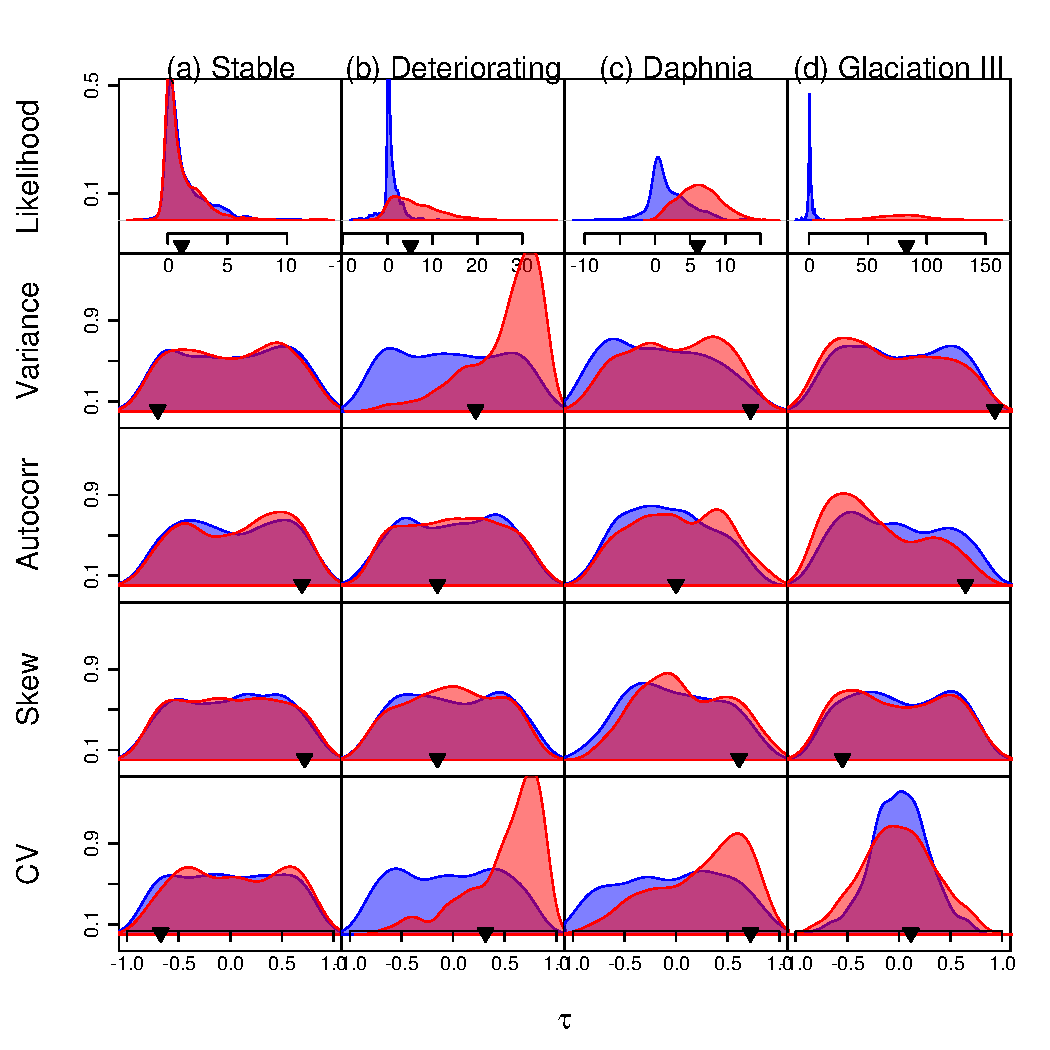
\includegraphics{FigS1.pdf}
  \end{center}
  \caption{Distribution of the indicator statistics corresponding to the ROC curves in Fig. 3, main text. As in Fig. 1, the expected distribution of the statistic under the null hypothesis of a stable system is shown in blue, while the distribution under the estimated deteriorating stability system is shown in red.  The value of the test statistic ($\delta$ in Likelihood, top row, otherwise $\tau$), observed in the original time-series is indicated by the black triangle. Distributions are produced from a Gaussian kernel density estimate from 500 replicates, as described in Methods.}
  \label{fig:S1}
\end{figure}

\begin{figure}[ht]
  \begin{center}
    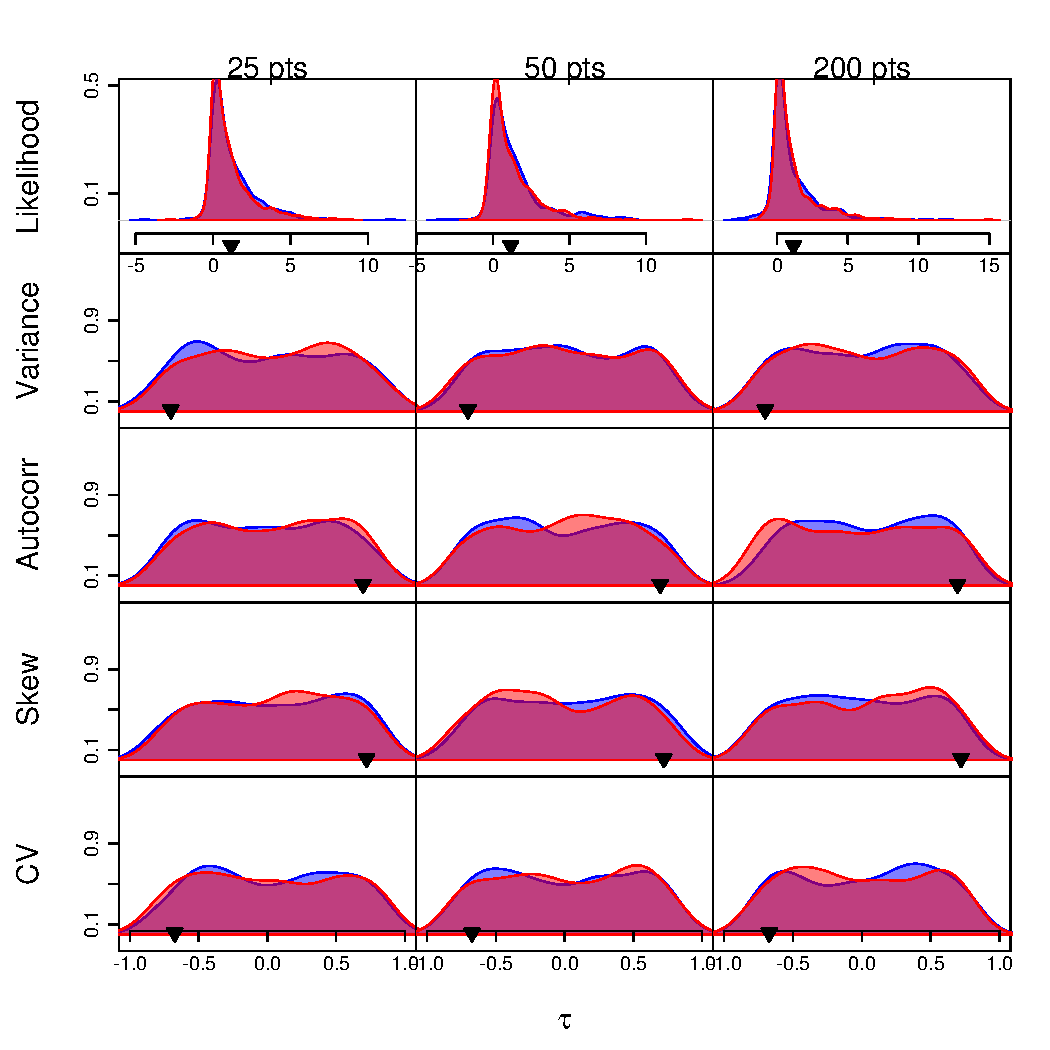
\includegraphics{FigS2.pdf}
  \end{center}
  \caption{Distributions of the indicator statistic as the sampling effort increases in the simulated data of a stable system, corresponding to the first column of Fig. 4, main text.  Distributions as described in caption of Fig~\ref{fig:S1}.}
  \label{fig:S2}
\end{figure}

\begin{figure}[ht]
  \begin{center}
    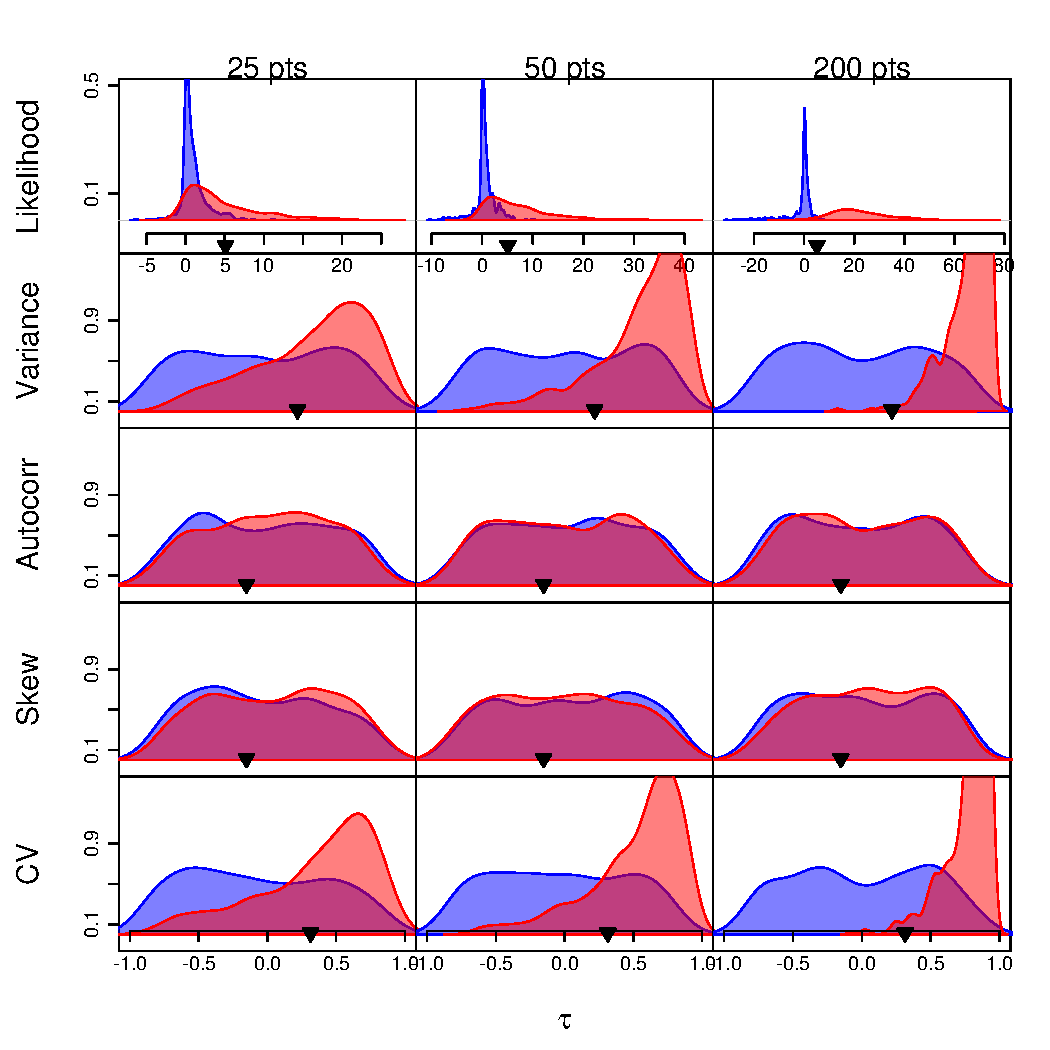
\includegraphics{FigS3.pdf}
  \end{center}
  \caption{Distributions of the indicator statistic as the sampling effort increases in the simulated data of a system under deteriorating stability, corresponding to the second column of Fig. 4, main text.  Distributions as described in caption of Fig~\ref{fig:S2}.}
  \label{fig:S3}
\end{figure}




\begin{figure}[ht]
  \begin{center}
    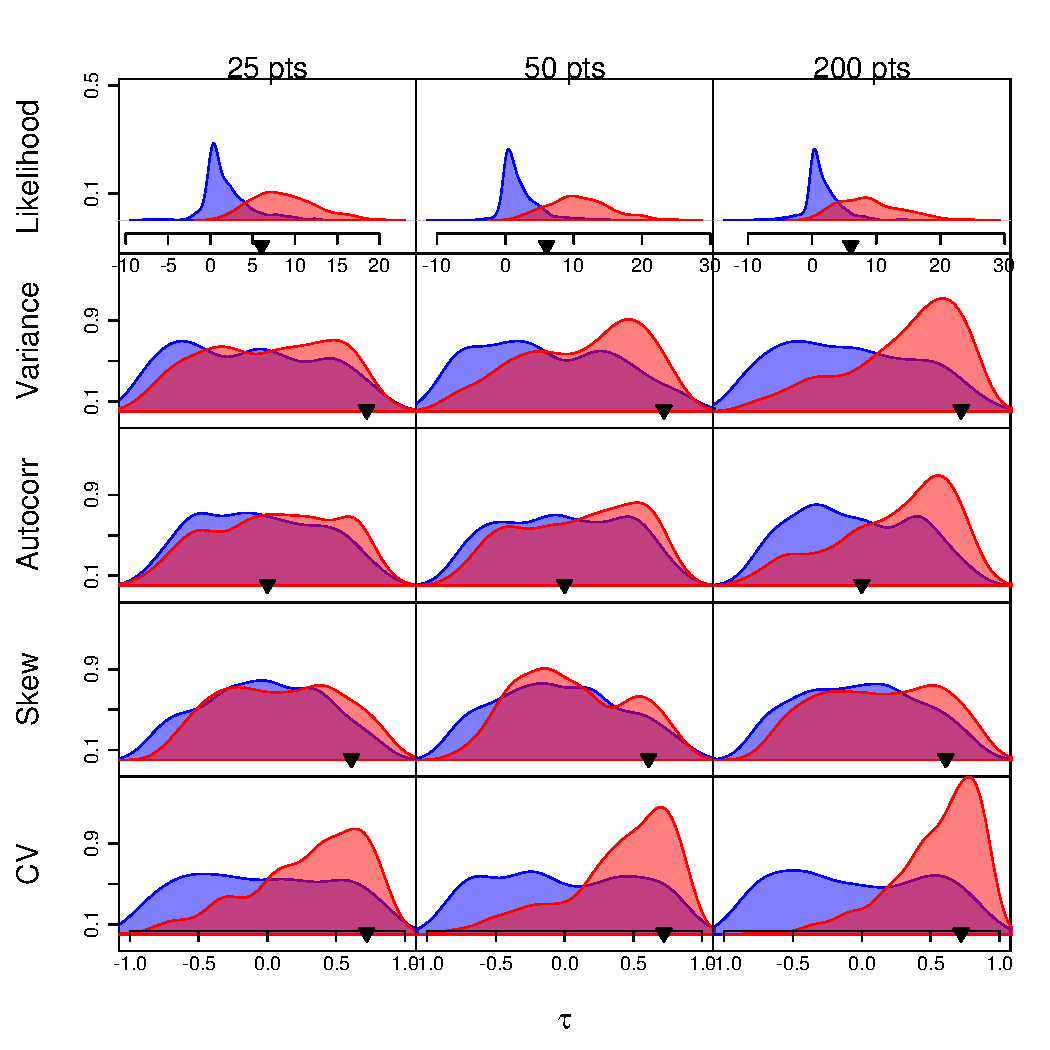
\includegraphics{FigS4.pdf}
  \end{center}
  \caption{Distributions of the indicator statistic as the sampling effort increases in the \emph{Daphnia} data, corresponding to the third column of Fig. 4, main text.  Distributions as described in caption of Fig~\ref{fig:S1}.}
  \label{fig:S4}
\end{figure}


\begin{figure}[ht]
  \begin{center}
    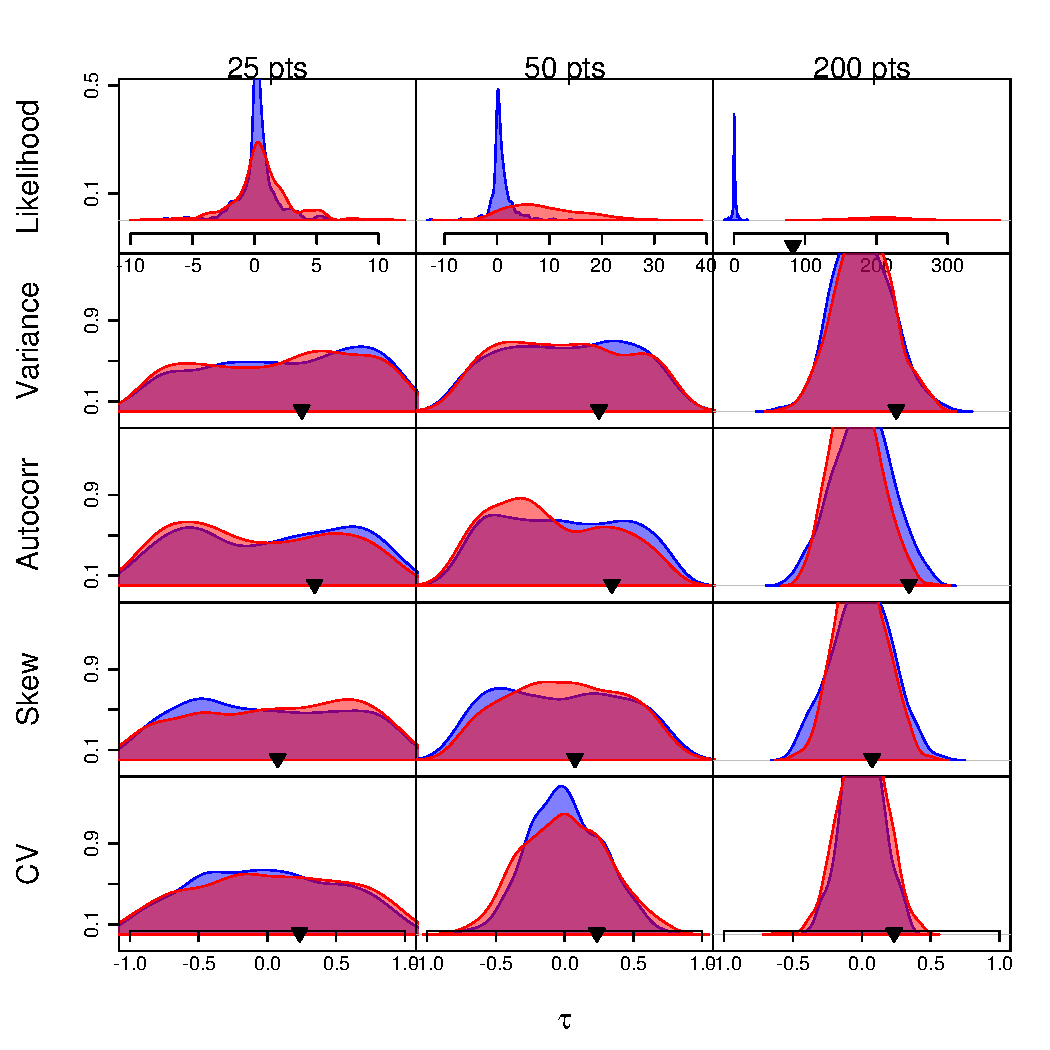
\includegraphics{FigS5.pdf}
  \end{center}
  \caption{Distributions of the indicator statistic as the sampling effort increases in the Glaciation data, corresponding to the fourth column of Fig. 4, main text.  Distributions as described in caption of Fig~\ref{fig:S1}.}
  \label{fig:S5}
\end{figure}

\pagebreak

\section*{ }%bibliography
 \bibliography{boettiger.bib}

 \end{document}



